\documentclass{article}\usepackage[]{graphicx}\usepackage[]{xcolor}
% maxwidth is the original width if it is less than linewidth
% otherwise use linewidth (to make sure the graphics do not exceed the margin)
\makeatletter
\def\maxwidth{ %
  \ifdim\Gin@nat@width>\linewidth
    \linewidth
  \else
    \Gin@nat@width
  \fi
}
\makeatother

\definecolor{fgcolor}{rgb}{0.345, 0.345, 0.345}
\newcommand{\hlnum}[1]{\textcolor[rgb]{0.686,0.059,0.569}{#1}}%
\newcommand{\hlstr}[1]{\textcolor[rgb]{0.192,0.494,0.8}{#1}}%
\newcommand{\hlcom}[1]{\textcolor[rgb]{0.678,0.584,0.686}{\textit{#1}}}%
\newcommand{\hlopt}[1]{\textcolor[rgb]{0,0,0}{#1}}%
\newcommand{\hlstd}[1]{\textcolor[rgb]{0.345,0.345,0.345}{#1}}%
\newcommand{\hlkwa}[1]{\textcolor[rgb]{0.161,0.373,0.58}{\textbf{#1}}}%
\newcommand{\hlkwb}[1]{\textcolor[rgb]{0.69,0.353,0.396}{#1}}%
\newcommand{\hlkwc}[1]{\textcolor[rgb]{0.333,0.667,0.333}{#1}}%
\newcommand{\hlkwd}[1]{\textcolor[rgb]{0.737,0.353,0.396}{\textbf{#1}}}%
\let\hlipl\hlkwb

\usepackage{framed}
\makeatletter
\newenvironment{kframe}{%
 \def\at@end@of@kframe{}%
 \ifinner\ifhmode%
  \def\at@end@of@kframe{\end{minipage}}%
  \begin{minipage}{\columnwidth}%
 \fi\fi%
 \def\FrameCommand##1{\hskip\@totalleftmargin \hskip-\fboxsep
 \colorbox{shadecolor}{##1}\hskip-\fboxsep
     % There is no \\@totalrightmargin, so:
     \hskip-\linewidth \hskip-\@totalleftmargin \hskip\columnwidth}%
 \MakeFramed {\advance\hsize-\width
   \@totalleftmargin\z@ \linewidth\hsize
   \@setminipage}}%
 {\par\unskip\endMakeFramed%
 \at@end@of@kframe}
\makeatother

\definecolor{shadecolor}{rgb}{.97, .97, .97}
\definecolor{messagecolor}{rgb}{0, 0, 0}
\definecolor{warningcolor}{rgb}{1, 0, 1}
\definecolor{errorcolor}{rgb}{1, 0, 0}
\newenvironment{knitrout}{}{} % an empty environment to be redefined in TeX

\usepackage{alltt}

\usepackage[utf8]{inputenc}
\usepackage{geometry}
\geometry{
paperwidth    = 210 mm,
paperheight   = 297 mm,
layoutwidth   = 210 mm,
layoutheight  = 297 mm,
layouthoffset = 5 mm,
layoutvoffset = 5 mm,
textwidth     = 150 mm,
textheight    = 200 mm,
includehead   = false,
includefoot   = false,
lmargin       = 25 mm,
rmargin       = 25 mm,
tmargin       = 25 mm,
bmargin       = 25 mm
}
\usepackage{amsmath}
\usepackage{parskip}
\usepackage{siunitx}
\usepackage{textcomp}
\usepackage{indentfirst}
\usepackage{graphicx}
\usepackage{float}
\usepackage{array}

\newenvironment{conditions}
  {\par\vspace{\abovedisplayskip}\noindent\begin{tabular}{>{$}l<{$} @{${}={}$} l}}
  {\end{tabular}\par\vspace{\belowdisplayskip}}
















\sisetup{
round-mode = places,
round-precision = 3
}
\title{Determinants of Interest Rates \\ [1ex] \large \textit{Term Structure of Interest Rates}}
\author{Emerson Maurício de Oliveira}

\IfFileExists{upquote.sty}{\usepackage{upquote}}{}
\begin{document}

\setlength{\abovedisplayskip}{0pt}
\setlength{\belowdisplayskip}{0pt}
\setlength{\abovedisplayshortskip}{0pt}
\setlength{\belowdisplayshortskip}{0pt}



\begin{center}
\Large
\textbf{Study Notes}\\
\vspace{0.5 cm}
\large
Financial Accounting: An Introduction to Concepts, Methods, and Uses, 14e\\
Roman Weil, Katherine Schipper, Jennifer Francis
\end{center}

\vspace{0.5 cm}

\textbf{Version Control System}\par

Date: 2022-10-13 19:48:00\\
Author: Emerson Maurício de Oliveira\\
Document name: saunders-fmi-c02-p14-r00\\
Document description: solution of the problem 14 chapter 2.\par

% -----------------------------------------------------------------------------------------------
\textbf{Problem Statement}\par
% -----------------------------------------------------------------------------------------------
Based on economists' forecasts and analysis, one-year Treasury bill rates and liquidity premiums 
for the next four years are expected to be as follows:

\begin{flalign*}
&	\text{Current 1-Year Treasury Bill Rate}		                      & {}^{}_{1}R^{}_{1}     &=  5.65\% 	& \\
&	\text{Expected 1-Year Treasury Bill Rate 1-Year from today}	      & E({}^{}_{2}r^{}_{1})  &=  6.75\% 	& \\
&	\text{Expected 1-Year Treasury Bill Rate 2-Year from today}	      & E({}^{}_{3}r^{}_{1})  &=  6.85\% 	& \\
&	\text{Expected 1-Year Treasury Bill Rate 3-Year from today}	      & E({}^{}_{4}r^{}_{1})  &=  7.15\% 	& \\
&	\text{Liquidity Premium for 1-Year T-Bill Rate 1-Year from today}	& L_2                   &=  0.05\% 	& \\
&	\text{Liquidity Premium for 1-Year T-Bill Rate 2-Year from today}	& L_3                   &=  0.10\% 	& \\
&	\text{Liquidity Premium for 1-Year T-Bill Rate 3-Year from today}	& L_4                   &=  0.12\% 	& \\
\end{flalign*}

Using the liquidity premium theory, plot the current yield curve. Make sure you label the axes on 
the graph and identify the four annual rates on the curve both on the axes and on the yield curve itself.

% -----------------------------------------------------------------------------------------------
\textbf{Assumptions}\par
% -----------------------------------------------------------------------------------------------
long-term rates are equal to geometric averages of current and expected short-term rates, plus 
liquidity risk premiums that increase with the security’s maturity. (Liquidity premium theory).\par
% -----------------------------------------------------------------------------------------------
\textbf{Solution}\par
% -----------------------------------------------------------------------------------------------
Data input:\par
\begin{knitrout}
\definecolor{shadecolor}{rgb}{0.969, 0.969, 0.969}\color{fgcolor}\begin{kframe}
\begin{alltt}
\hlstd{c1yTb1y} \hlkwb{<-} \hlnum{0.0565}
\hlstd{e1yTb2y} \hlkwb{<-} \hlnum{0.0675}
\hlstd{e1yTb3y} \hlkwb{<-} \hlnum{0.0685}
\hlstd{e1yTb4y} \hlkwb{<-} \hlnum{0.0715}
\hlstd{liqPr2y} \hlkwb{<-} \hlnum{0.0005}
\hlstd{liqPr3y} \hlkwb{<-} \hlnum{0.0010}
\hlstd{liqPr4y} \hlkwb{<-} \hlnum{0.0012}
\end{alltt}
\end{kframe}
\end{knitrout}
Calculations:\par
\begin{knitrout}
\definecolor{shadecolor}{rgb}{0.969, 0.969, 0.969}\color{fgcolor}\begin{kframe}
\begin{alltt}
\hlcom{# Current 1-year T-bill rate 1-year from today}
\hlstd{c1yTb2y} \hlkwb{<-} \hlstd{( ( (} \hlnum{1} \hlopt{+} \hlstd{c1yTb1y )} \hlopt{*}
               \hlstd{(} \hlnum{1} \hlopt{+} \hlstd{e1yTb2y} \hlopt{+} \hlstd{liqPr2y ) )} \hlopt{^} \hlstd{(} \hlnum{1} \hlopt{/} \hlnum{2} \hlstd{) )} \hlopt{-} \hlnum{1}
\hlcom{# Current 1-year T-bill rate 2-year from today}
\hlstd{c1yTb3y} \hlkwb{<-} \hlstd{( ( (} \hlnum{1} \hlopt{+} \hlstd{c1yTb1y )} \hlopt{*}
               \hlstd{(} \hlnum{1} \hlopt{+} \hlstd{e1yTb2y} \hlopt{+} \hlstd{liqPr2y )} \hlopt{*}
               \hlstd{(} \hlnum{1} \hlopt{+} \hlstd{e1yTb3y} \hlopt{+} \hlstd{liqPr3y ) )} \hlopt{^} \hlstd{(} \hlnum{1} \hlopt{/} \hlnum{3} \hlstd{) )} \hlopt{-} \hlnum{1}
\hlcom{# Current 1-year T-bill rate 3-year from today}
\hlstd{c1yTb4y} \hlkwb{<-} \hlstd{( ( (} \hlnum{1} \hlopt{+} \hlstd{c1yTb1y )} \hlopt{*}
               \hlstd{(} \hlnum{1} \hlopt{+} \hlstd{e1yTb2y} \hlopt{+} \hlstd{liqPr2y )} \hlopt{*}
               \hlstd{(} \hlnum{1} \hlopt{+} \hlstd{e1yTb3y} \hlopt{+} \hlstd{liqPr3y )} \hlopt{*}
               \hlstd{(} \hlnum{1} \hlopt{+} \hlstd{e1yTb4y} \hlopt{+} \hlstd{liqPr4y ) )} \hlopt{^} \hlstd{(} \hlnum{1} \hlopt{/} \hlnum{4} \hlstd{) )} \hlopt{-} \hlnum{1}
\end{alltt}
\end{kframe}
\end{knitrout}
Results:\par
\begin{itemize}
  \item Current 1-Year Treasury Bill Rate: \num{5.65}\%.
  \item Current 1-Year Treasury Bill Rate 1 year from today: \num{6.2234437}\%.
  \item Current 1-Year Treasury Bill Rate 2 year from today: \num{6.4650791}\%.
  \item Current 1-Year Treasury Bill Rate 3 year from today: \num{6.6657413}\%.
\end{itemize}
Yield curve:\par
\begin{knitrout}
\definecolor{shadecolor}{rgb}{0.969, 0.969, 0.969}\color{fgcolor}

{\centering 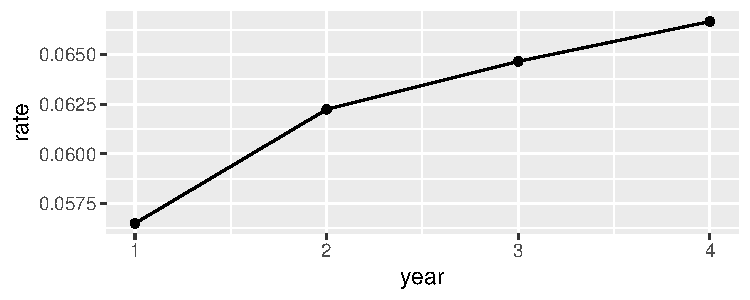
\includegraphics[width=\maxwidth]{figure/plot-1} 

}


\end{knitrout}



% --------------------------------------------------------------------------------

% \begin{flalign*}
% &	\text{Current 1-Year Treasury Bill Rate}		                      & {}^{}_{1}R^{}_{1}     &=  5.65\% 	& \\
% &	\text{Expected 1-Year Treasury Bill Rate 1-Year from today}	      & E({}^{}_{2}r^{}_{1})  &=  6.75\% 	& \\
% &	\text{Expected 1-Year Treasury Bill Rate 2-Year from today}	      & E({}^{}_{3}r^{}_{1})  &=  6.85\% 	& \\
% &	\text{Expected 1-Year Treasury Bill Rate 3-Year from today}	      & E({}^{}_{4}r^{}_{1})  &=  7.15\% 	& \\
% &	\text{Liquidity Premium for 1-Year T-Bill Rate 1-Year from today}	& L_2                   &=  0.05\% 	& \\
% &	\text{Liquidity Premium for 1-Year T-Bill Rate 2-Year from today}	& L_3                   &=  0.10\% 	& \\
% &	\text{Liquidity Premium for 1-Year T-Bill Rate 3-Year from today}	& L_4                   &=  0.12\% 	& \\
% \end{flalign*}

%(1+{}^{}_{1}R^{}_{4})^4&=(1+{}^{}_{1}R^{}_{1})(1+E({}^{}_{2}r^{}_{1}))(1+E({}^{}_{3}r^{}_{1}))(1+E({}^{}_{4}r^{}_{1}))
\end{document}
